\clearpage

\subsection{Opaque without Survivability}\label{ILP_Opaque_Survivability}
\begin{tcolorbox}	
\begin{tabular}{p{2.75cm} p{0.2cm} p{10.5cm}} 	
\textbf{Student Name}  &:& Tiago Esteves    (October 03, 2017 - )\\
\textbf{Goal}          &:& Implement the ILP model for the opaque transport mode without survivability.
\end{tabular}
\end{tcolorbox}

\subsubsection{Model description}

First, for a better understanding of the functions and variables used in the ILP, a table \ref{description_opaque} will be created with all indexes, inputs and variables and with their respective description.\\

\begin{table}[h!]
\centering
\begin{tabular}{ |p{1cm}||p{13cm}|}
 \hline
 \multicolumn{2}{|c|}{Description of notation used in the objective function} \\
 \hline
 \hline
 $i$ & index for start node of a physical link \\
 $j$ & index for end node of a physical link \\
 $o$ & index for node that is origin of a demand \\
 $d$ & index for node that is destination of a demand \\
 $c$ & index for bit rate of the client signal \\
 $($ i,j $)$ & physical link between the nodes $i$ and $j$ \\
 $($ o,d $)$ & demand between the nodes $o$ and $d$ \\
 $C$ & set of the client signal \\
 $f_{ij}^{od}$ & binary variable indicating if link between the nodes $i$ and $j$ is used in the path between nodes $o$ and $d$ \\
 $L_{ij}$ & binary variable indicating if link between the nodes $i$ and $j$ is used \\
 $W_{ij}$ & number of optical channels between the nodes $i$ and $j$\\
 $B_c $ & client signals granularities $($1.25, 2.5, 10, 40, 100$)$ \\
 $D_{odc}$ & client demands between nodes $o$ and $d$ with bit rate $c$\\
 $G_{ij}$ & network topology in form of adjacency matrix \\
 \hline
\end{tabular}
\caption{Table with description of variables used in opaque transport mode.}
\label{description_opaque}
\end{table}

Before carrying out the description of the objective function we must take into account the following particularity of this mode of transport:
\begin{itemize}
  \item $N_{OXC,n}$ = 0, \quad $\forall$ n
  \item $N_{EXC,n}$ = 1, \quad $\forall$ n that process traffic
\end{itemize}

\vspace{11pt}
The objective function of following the ILP is a minimization of the CAPEX through the equation \ref{Capex} where in this case for the cost of nodes we only have in consideration the electric cost \ref{Capex_Node_EXC} because of the particularity previously mentioned.
In this case the value of $P_{exc,c,n}$ is obtained by equation \ref{EXC_pexc1_opaque} for long-reach and by the equation \ref{EXC_pexc2_opaque} for short-reach.\\

\newpage
As previously mentioned, equation \ref{EXC_pexc1_opaque} refers to the number of long-reach ports of the electrical switch with bit-rate -1 in node n, $P_{exc,-1,n}$, i.e. the number of line ports of node n which can be calculated as

\begin{equation}
P_{exc,-1,n} = \sum_{j=1}^{N} w_{nj}
\label{EXC_pexc1_opaque}
\end{equation}
\vspace{11pt}

\noindent
where $w_{nj}$ is the number of optical channels between node $n$ and node $j$.\\

As previously mentioned, equation \ref{EXC_pexc2_opaque} refers to the number of sort-reach ports of the electrical switch with bit-rate c in node n, $P_{exc,c,n}$, i.e. the number of tributary ports with bit-rate c in node n which can be calculated as

\begin{equation}
P_{exc,c,n} = \sum_{d=1}^{N} D_{nd,c}
\label{EXC_pexc2_opaque}
\end{equation}

\vspace{11pt}
\noindent
where $D_{nd,c}$ are the client demands between nodes $n$ and $d$ with bit rate $c$.\\

In this case there is the following particularity:

\begin{itemize}
  \item When $n$=$d$ the value of client demands is always zero, i.e, $D_{nn,c}=0$
\end{itemize}


\vspace{17pt}
The objective function, to be minimized, is the expression \ref{ILPOpaque_CAPEX}, i.e.,
\begin{equation*}
  minimize \qquad \Big\{ \quad C_C \quad \Big\}
\end{equation*}

$subject$ $to$
\begin{equation}
\sum_{j\textbackslash \{o\}} f_{ij}^{od} = 1  \qquad \qquad \qquad \qquad \qquad \qquad \qquad \qquad \qquad \qquad
\forall(o,d) : o < d, \forall i: i = o
\label{ILPOpaque1_Surv}
\end{equation}
\noindent
This constraint are equal to the constraint \ref{ILPOpaque1_CAPEX} assuming that Z variable has the value of 1.

\begin{equation}
\sum_{j\textbackslash \{o\}} f_{ij}^{od} = \sum_{j\textbackslash \{d\}} f_{ji}^{od}   \qquad \qquad \qquad \qquad \qquad \qquad \qquad \qquad
\forall(o,d) : o < d, \forall i: i \neq o,d
\label{ILPOpaque2_Surv}
\end{equation}
\noindent
This constraint are equal to the constraint \ref{ILPOpaque2_CAPEX}.

\begin{equation}
\sum_{j\textbackslash \{d\}} f_{ji}^{od} = 1  \qquad \qquad \qquad \qquad \qquad \qquad \qquad \qquad \qquad \qquad
\forall(o,d) : o < d, \forall i: i = d
\label{ILPOpaque3_Surv}
\end{equation}
\noindent
This constraint are equal to the constraint \ref{ILPOpaque3_CAPEX} assuming that Z variable has the value of 1.
\newpage
\begin{equation}
\sum_{o=1} \sum_{d=o+1} \left(f_{ij}^{od} + f_{ji}^{od}\right) \sum_{c\in C} (B\left(c\right) D_{odc}\leq \tau W_{ij} G_{ij} \qquad \qquad \qquad \qquad
\forall(i,j) : i < j
\label{ILPOpaque4_Surv}
\end{equation}
\noindent
This restriction is considered grooming constraint, so it means the total client traffic flows can not be greater than the capacity of optical transmission system on all links where $\tau$ is always 100 Gbits/s.

\begin{equation}
W_{ij} \leq K_{ij} L_{ij} \qquad  \qquad \qquad \qquad \qquad \qquad \qquad \qquad \qquad \qquad \qquad \qquad \forall(i,j) : i < j
\label{ILPOpaque5_Surv}
\end{equation}
\noindent
This restriction concerns the capacity of the optical channels which must be less or equal to the maximum number of optical channels. For any situation the maximum number of optical channels supported by each transmission system is 100, i.e., $K_{ij}$ = 100.

\begin{equation}
f_{ij}^{od} , f_{ji}^{od} \in \{0,1\}   \qquad \qquad \qquad \qquad \qquad \qquad \qquad \qquad
\forall(i,j) : i < j, \forall(o,d) : o < d
\label{ILPOpaque6_Surv}
\end{equation}
\noindent
The number of flows per demand in this case can be zero if there are no traffic demands or one if considering traffic.

\begin{equation}
W_{ij} \in \mathbb{N}  \qquad \qquad \qquad \qquad \qquad \qquad \qquad \qquad \qquad \qquad \qquad \qquad \qquad
\forall(i,j) : i < j
\label{ILPOpaque7_Surv}
\end{equation}
\noindent
The last constraint is just needed to ensure the number optical of channels is a positive integer values greater than zero.


\subsubsection{Result description}

To perform the calculations using the implementation of the models described previously it is necessary to use a mathematical software tool. For this we will use MATLAB which is ideal for dealing with linear programming problems and can call the LPsolve through an external interface.
We already have all the necessary to obtain the CAPEX value for the reference network \ref{Reference_Network_Topology}. As described in the subsection of network traffic \ref{Reference_Network_Traffic}, we have three values of network traffic (low, medium and high traffic) so we have to obtain three different CAPEX.
The value of the CAPEX of the network will be calculated based on the costs of the equipment present in the table \ref{table_cost_ilp}.\\


\textbf{Low Traffic Scenario:}\\

In this scenario we have to take into account the traffic calculated in \ref{low_scenario}. In a first phase we will show the various existing topologies of the network. The first are the allowed topologies, physical and optical topology, the second are the logical topology for all ODUs and finally the resulting physical and optical topology.\\

\newpage
\vspace{20pt}
\begin{figure}[h!]
\centering
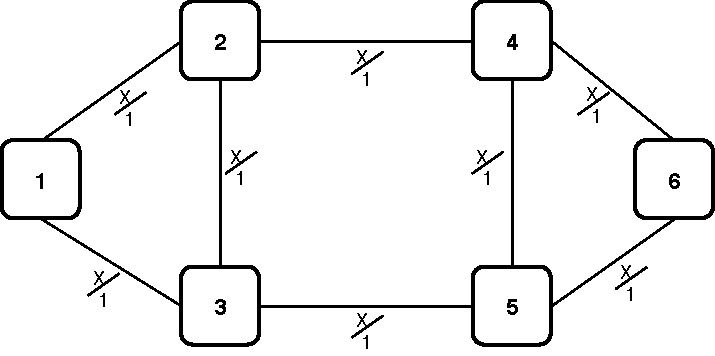
\includegraphics[width=13cm]{sdf/ilp/opaque_survivability/figures/allowed_physical_topology}
\caption{Allowed physical topology. The allowed physical topology is defined by the duct and sites in the field. It is assumed that each duct supports up to 1 bidirectional transmission system and each site supports up to 1 node.}
\label{allowed_physical_low}
\end{figure}

\vspace{20pt}
\begin{figure}[h!]
\centering
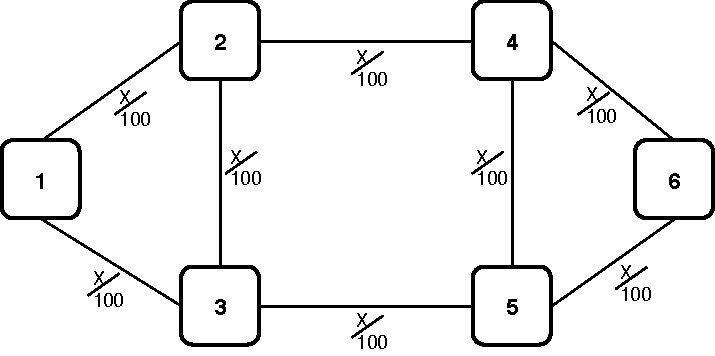
\includegraphics[width=13cm]{sdf/ilp/opaque_survivability/figures/allowed_optical_topology}
\caption{Allowed optical topology. The allowed optical topology is defined by the transport mode (opaque transport mode in this case). It is assumed that each transmission system supports up to 100 optical channels.}
\label{allowed_optical_low}
\end{figure}

\newpage
\begin{figure}[h!]
\centering
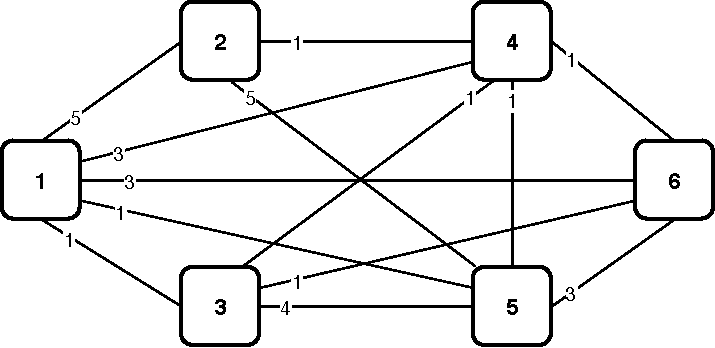
\includegraphics[width=12cm]{sdf/ilp/opaque_survivability/figures/logical_topology_ODU0_low}
\caption{ODU0 logical topology defined by the ODU0 traffic matrix.}
\label{logical_ODU0_low}
\end{figure}

\begin{figure}[h!]
\centering
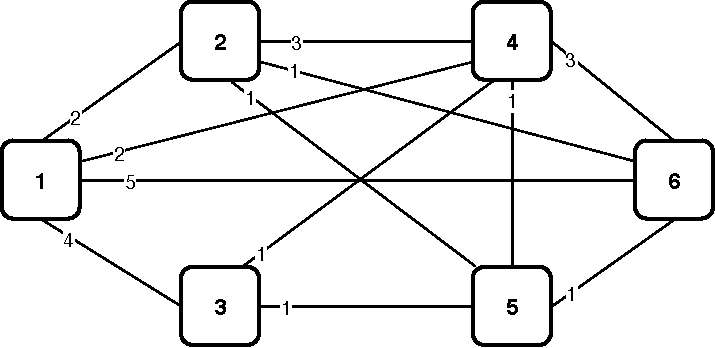
\includegraphics[width=12cm]{sdf/ilp/opaque_survivability/figures/logical_topology_ODU1_low}
\caption{ODU1 logical topology defined by the ODU1 traffic matrix.}
\label{logical_ODU1_low}
\end{figure}

\begin{figure}[h!]
\centering
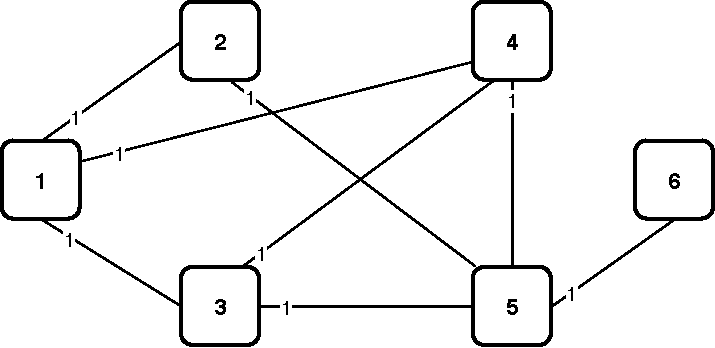
\includegraphics[width=12cm]{sdf/ilp/opaque_survivability/figures/logical_topology_ODU2_low}
\caption{ODU2 logical topology defined by the ODU2 traffic matrix.}
\label{logical_ODU2_low}
\end{figure}

\begin{figure}[h!]
\centering
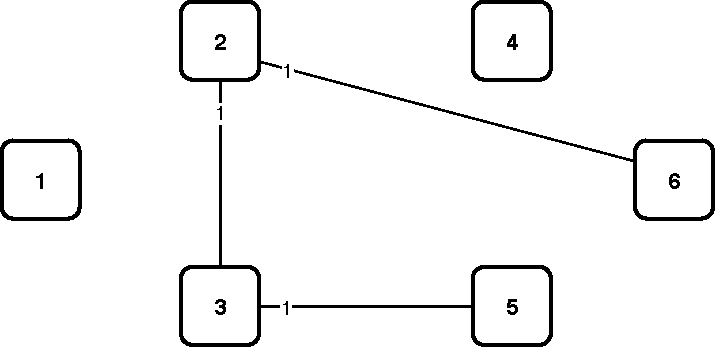
\includegraphics[width=12cm]{sdf/ilp/opaque_survivability/figures/logical_topology_ODU3_low}
\caption{ODU3 logical topology defined by the ODU3 traffic matrix.}
\label{logical_ODU3_low}
\end{figure}

\begin{figure}[h!]
\centering
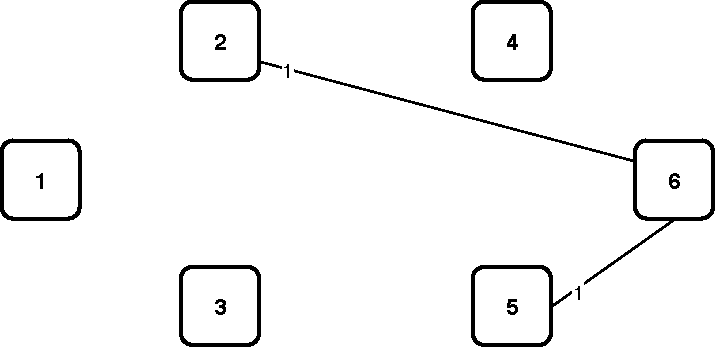
\includegraphics[width=12cm]{sdf/ilp/opaque_survivability/figures/logical_topology_ODU4_low}
\caption{ODU4 logical topology defined by the ODU4 traffic matrix.}
\label{logical_ODU4_low}
\end{figure}

\begin{figure}[h!]
\centering
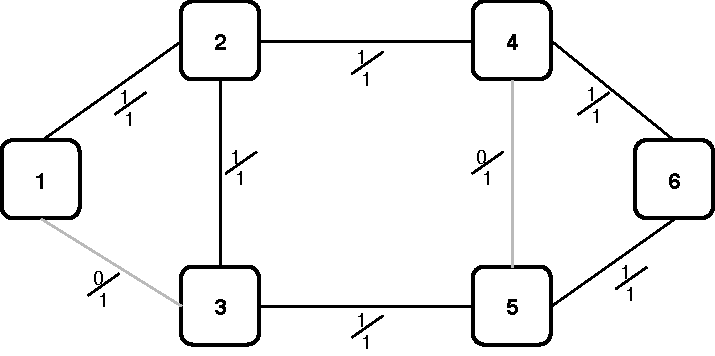
\includegraphics[width=12cm]{sdf/ilp/opaque_survivability/figures/physical_topology_low}
\caption{Physical topology after dimensioning.}
\label{physical_low}
\end{figure}

\begin{figure}[h!]
\centering
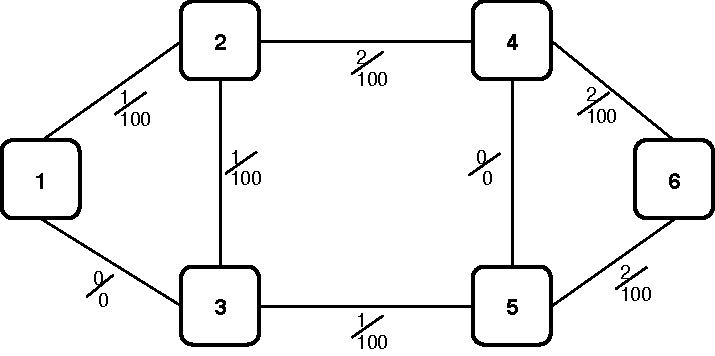
\includegraphics[width=13cm]{sdf/ilp/opaque_survivability/figures/optical_topology_low}
\caption{Optical topology after dimensioning.}
\label{optical_low}
\end{figure}

\vspace{15pt}
In table \ref{link_opaque_surv_ref_low} we can see the number of optical channels calculated using \ref{Capex_Link} and \ref{ILPOpaque_CAPEX} and the number of amplifiers for each link calculated using \ref{Capex_amplifiers}. In the case where there are no optical channels we assume that the number of amplifiers is zero.\\

\begin{table}[h!]
\centering
\begin{tabular}{|| c | c | c ||}
 \hline
 \multicolumn{3}{|| c ||}{Information regarding links} \\
 \hline
 \hline
 Bidirectional Link & Optical Channels & Amplifiers\\
 \hline
 Node 1 <-> Node 2 & 1 & 4 \\
 Node 1 <-> Node 3 & 0 & 0 \\
 Node 2 <-> Node 3 & 1 & 0 \\
 Node 2 <-> Node 4 & 2 & 6 \\
 Node 3 <-> Node 5 & 1 & 8 \\
 Node 4 <-> Node 5 & 0 & 0 \\
 Node 4 <-> Node 6 & 2 & 7 \\
 Node 5 <-> Node 6 & 2 & 3 \\
 \hline
\end{tabular}
\caption{Table with information regarding links for opaque mode without survivability.}
\label{link_opaque_surv_ref_low}
\end{table}

\vspace{15pt}
In table \ref{node_opaque_surv_ref_low} we can see the resulting nodal degree at the physical layer, calculated based on the number of connections that the node in question performs, the number of line ports calculated using \ref{EXC_pexc1_opaque} and the number of tributary ports calculated using \ref{EXC_pexc2_opaque} for each node.\\
\newpage
\begin{table}[h!]
\centering
\begin{tabular}{|| c | c | c | c ||}
 \hline
 \multicolumn{4}{|| c ||}{Information regarding nodes} \\
 \hline
 \hline
 Node & Resulting Nodal Degree & Line Ports & Tributary Ports\\
 \hline
 1 & 1 & 1 & 29 \\
 2 & 3 & 4 & 23 \\
 3 & 2 & 2 & 18 \\
 4 & 2 & 4 & 20 \\
 5 & 2 & 3 & 24 \\
 6 & 2 & 4 & 22 \\
\hline
\end{tabular}
\caption{Table with information regarding nodes for opaque mode without survivability.}
\label{node_opaque_surv_ref_low}
\end{table}

Through the information obtained previously on the nodes we can now create tables with detailed information about each node. In each table mentioned below we can see how many ports are connected to a given node and its bit rate (in relation to the line ports) and how many ports are assigned to each different bit rate (in relation to the tributary ports).

\begin{table}[h!]
\centering
\begin{tabular}{|| c | c | c ||}
 \hline
 \multicolumn{3}{|| c ||}{Detailed description of Node 1} \\
 \hline
 \hline
  & Number of total demands & Bit rate \\
 \hline
 \multirow{3}{*}{29 tributary ports} & 13 & ODU0 \\
 & 13 & ODU1 \\
 & 3 & ODU2 \\
 \hline
 \hline
  & Node<--Optical Channels-->Node & Bit rate \\
 \hline
 1 line ports & 1  <---- 1 ---->  2 & 100 Gbits/s \\
\hline
\end{tabular}
\caption{Table with detailed description of node 1. The number of demands is distributed to the various destination nodes, this distribution can be observed in section \ref{low_scenario}.}
\end{table}

\begin{table}[h!]
\centering
\begin{tabular}{|| c | c | c ||}
 \hline
 \multicolumn{3}{|| c ||}{Detailed description of Node 2} \\
 \hline
 \hline
  & Number of total demands & Bit rate \\ \hline
 \multirow{5}{*}{23 tributary ports} & 11 & ODU0 \\
 & 7 & ODU1 \\
 & 2 & ODU2 \\
 & 2 & ODU3 \\
 & 1 & ODU4 \\
 \hline
 \hline
  & Node<--Optical Channels-->Node & Bit rate \\ \hline
 \multirow{3}{*}{4 line ports} & 2  <---- 1 ---->  1 & \multirow{3}{*}{100 Gbits/s} \\
 & 2  <---- 1 ---->  3 & \\
 & 2  <---- 2 ---->  4 & \\
\hline
\end{tabular}
\caption{Table with detailed description of node 2. The number of demands is distributed to the various destination nodes, this distribution can be observed in section \ref{low_scenario}.}
\end{table}

\newpage
\begin{table}[h!]
\centering
\begin{tabular}{|| c | c | c ||}
 \hline
 \multicolumn{3}{|| c ||}{Detailed description of Node 3} \\
 \hline
 \hline
  & Number of total demands & Bit rate \\ \hline
 \multirow{4}{*}{18 tributary ports} & 7 & ODU0 \\
 & 6 & ODU1\\
 & 3 & ODU2\\
 & 2 & ODU3\\
 \hline
 \hline
  & Node<--Optical Channels-->Node & Bit rate \\
 \hline
 \multirow{2}{*}{2 line ports} & 3  <---- 1 ---->  2 & \multirow{2}{*}{100 Gbits/s}\\
 & 3  <---- 1 ---->  5 & \\
\hline
\end{tabular}
\caption{Table with detailed description of node 3. The number of demands is distributed to the various destination nodes, this distribution can be observed in section \ref{low_scenario}.}
\end{table}

\vspace{13pt}
\begin{table}[h!]
\centering
\begin{tabular}{|| c | c | c ||}
 \hline
 \multicolumn{3}{|| c ||}{Detailed description of Node 4} \\
 \hline
 \hline
  & Number of total demands & Bit rate \\ \hline
 \multirow{3}{*}{20 tributary ports} & 7 & ODU0 \\
 & 10 & ODU1 \\
 & 3 & ODU2 \\
 \hline
 \hline
  & Node<--Optical Channels-->Node & Bit rate \\
 \hline
 \multirow{2}{*}{4 line ports} & 4  <---- 2 ---- >  2 & \multirow{2}{*}{100 Gbits/s}\\
 & 4  <---- 2 ----> 6 & \\
\hline
\end{tabular}
\caption{Table with detailed description of node 4. The number of demands is distributed to the various destination nodes, this distribution can be observed in section \ref{low_scenario}.}
\end{table}

\vspace{13pt}
\begin{table}[h!]
\centering
\begin{tabular}{|| c | c | c ||}
 \hline
 \multicolumn{3}{|| c ||}{Detailed description of Node 5} \\
 \hline
 \hline
  & Number of total demands & Bit rate \\ \hline
 \multirow{5}{*}{24 tributary ports} & 14 & ODU0 \\
 & 4 & ODU1 \\
 & 4 & ODU2 \\
 & 1 & ODU3 \\
 & 1 & ODU4 \\
 \hline
 \hline
  & Node<--Optical Channels-->Node & Bit rate \\
 \hline
 \multirow{2}{*}{3 line ports} & 5  <---- 1 ---->  3 & \multirow{2}{*}{100 Gbits/s}\\
 & 5  <---- 2 ---->  6 & \\
 \hline
\end{tabular}
\caption{Table with detailed description of node 5. The number of demands is distributed to the various destination nodes, this distribution can be observed in section \ref{low_scenario}.}
\end{table}

\newpage
\begin{table}[h!]
\centering
\begin{tabular}{|| c | c | c ||}
 \hline
 \multicolumn{3}{|| c ||}{Detailed description of Node 6} \\
 \hline
 \hline
  & Number of total demands & Bit rate \\
 \hline
 \multirow{5}{*}{22 tributary ports} & 8 & ODU0 \\
 & 10 & ODU1 \\
 & 1 & ODU2 \\
 & 1 & ODU3 \\
 & 2 & ODU4 \\
 \hline
 \hline
  & Node<--Optical Channels-->Node & Bit rate \\
 \hline
 \multirow{2}{*}{4 line ports} & 6  <---- 2 ---->  4 & \multirow{2}{*}{100 Gbits/s}\\
 & 6  <---- 2 ---->  5 & \\
\hline
\end{tabular}
\caption{Table with detailed description of node 6. The number of demands is distributed to the various destination nodes, this distribution can be observed in section \ref{low_scenario}.}
\end{table}

\vspace{17pt}
In next step let's focus on the routing information. These paths are bidirectional so the path from one node to another is the same path in the opposite direction. In table \ref{path_opaque_surv_ref_low} we can see all the routing obtained for all nodes.\\

\begin{table}[h!]
\centering
\begin{tabular}{|| c | c | c | c | c | c | c | c ||}
 \hline
 \multicolumn{8}{|| c ||}{Routing} \\
 \hline
 \hline
 o & d & Links & ODU0 & ODU1 & ODU2 & ODU3 & ODU4 \\
 \hline
 1 & 2 & \{(1,2)\} & 5 & 2 & 1 & 0 & 0 \\ \hline
 1 & 3 & \{(1,2),(2,3)\} & 1 & 4 & 1 & 0 & 0\\ \hline
 1 & 4 & \{(1,2),(2,4)\} & 3 & 2 & 1 & 0 & 0\\ \hline
 1 & 5 & \{(1,2),(2,3),(3,5)\} & 1 & 0 & 0 & 0 & 0\\ \hline
 1 & 6 & \{(1,2),(2,4),(4,6)\} & 3 & 5 & 0 & 0 & 0\\ \hline
 2 & 3 & \{(2,3)\} & 0 & 0 & 0 & 1 & 0 \\ \hline
 2 & 4 & \{(2,4)\} & 1 & 3 & 0 & 0 & 0\\ \hline
 2 & 5 & \{(2,3),(3,5)\} & 5 & 1 & 1 & 0 & 0 \\ \hline
 2 & 6 & \{(2,4),(4,6)\} & 0 & 1 & 0 & 1 & 1 \\ \hline
 3 & 4 & \{(3,2),(2,4)\} & 1 & 1 & 1 & 0 & 0 \\ \hline
 3 & 5 & \{(3,5)\} & 4 & 1 & 1 & 1 & 0 \\ \hline
 3 & 6 & \{(3,5),(5,6)\} & 1 & 0 & 0 & 0 & 0\\ \hline
 4 & 5 & \{(4,6),(6,5)\} & 1 & 1 & 1 & 0 & 0\\ \hline
 4 & 6 & \{(4,6)\} & 1 & 3 & 0 & 0 & 0\\ \hline
 5 & 6 & \{(5,6)\} & 3 & 1 & 1 & 0 & 1\\
 \hline
\end{tabular}
\caption{Table with description of demands routing. We are assuming that between a pair of nodes all demands follow the same route.}
\label{path_opaque_surv_ref_low}
\end{table}

\newpage
Finally and most importantly through table \ref{scriptopaque_surv_ref_low} we can see the CAPEX result for this model. This value is obtained using equation \ref{ILPOpaque_CAPEX} and all of the constraints mentioned above.\\

\begin{table}[h!]
\centering
\begin{tabular}{|| c | c | c | c | c | c | c ||}
 \hline
 \multicolumn{7}{|| c ||}{CAPEX of the Network} \\
 \hline
 \hline
 \multicolumn{3}{|| c |}{ } & Quantity & Unit Price & Cost & Total \\
 \hline
 \multirow{3}{*}{Link Cost} & \multicolumn{2}{ c |}{OLTs} & 12 & 15 000 \euro & 180 000 \euro & \multirow{3}{*}{9 404 000 \euro} \\ \cline{2-6}
 & \multicolumn{2}{ c |}{100 Gbits/s Transceivers} & 18 & 5 000 \euro/Gbit/s & 9 000 000 \euro & \\ \cline{2-6}
 & \multicolumn{2}{ c |}{Amplifiers} & 56 & 4 000 \euro & 224 000 \euro & \\
 \hline
 \multirow{9}{*}{Node Cost} & \multirow{7}{*}{Electrical} & EXCs & 6 & 10 000 \euro & 60 000 \euro & \multirow{9}{*}{1 862 590 \euro} \\ \cline{3-6}
 & & ODU0 Ports & 60 & 10 \euro/port & 600 \euro & \\ \cline{3-6}
 & & ODU1 Ports & 50 & 15 \euro/port & 750 \euro & \\ \cline{3-6}
 & & ODU2 Ports & 16 & 30 \euro/port & 480 \euro & \\ \cline{3-6}
 & & ODU3 Ports & 6 & 60 \euro/port & 360 \euro & \\ \cline{3-6}
 & & ODU4 Ports & 4 & 100 \euro/port & 400 \euro & \\ \cline{3-6}
 & & Line Ports & 18 & 100 000 \euro/port & 1 800 000 \euro & \\ \cline{2-6}
 & \multirow{2}{*}{Optical} & OXCs & 0 & 20 000 \euro & 0 \euro & \\ \cline{3-6}
 & & Ports & 0 & 2 500 \euro/port & 0 \euro & \\
 \hline
 \multicolumn{6}{|| c |}{Total Network Cost} & 11 266 590 \euro \\
\hline
\end{tabular}
\caption{Table with detailed description of CAPEX for this scenario.}
\label{scriptopaque_surv_ref_low}
\end{table}

\vspace{17pt}
All the values calculated in the previous table were obtained through the equations \ref{Capex_Link} and \ref{Capex_Node} referred to in section \ref{ILP_CAPEX}, but for a more detailed analysis we created table \ref{formulas_opaque} where we can see how all the parameters are calculated individually.\\
\newpage
\begin{table}[h!]
\centering
\begin{tabular}{|| c | c ||}
 \hline
  & Equation used to calculate the cost \\ \hline
 OLTs & \(\displaystyle 2 \sum_{i=1}^{N}\sum_{j=i+1}^{N} L_{ij} \gamma_0^{OLT} \) \\ \hline
 Transceivers & \(\displaystyle 2 \sum_{i=1}^{N}\sum_{j=i+1}^{N} L_{ij} w_{ij} \gamma_1^{OLT} \tau \) \\ \hline
 Amplifiers & \(\displaystyle 2 \sum_{i=1}^{N}\sum_{j=i+1}^{N} L_{ij} N^R_{ij} c^R \) \\ \hline
 EXCs & \(\displaystyle \sum_{n=1}^N N_{exc,n} \gamma_{e0} \) \\ \hline
 ODU0 Port & \(\displaystyle \sum_{n=1}^{N} \sum_{d=1}^{N} N_{exc,n} D_{nd,0} \gamma_{e1,0} \) \\ \hline
 ODU1 Port & \(\displaystyle \sum_{n=1}^{N} \sum_{d=1}^{N} N_{exc,n} D_{nd,1} \gamma_{e1,1} \) \\ \hline
 ODU2 Port & \(\displaystyle \sum_{n=1}^{N} \sum_{d=1}^{N} N_{exc,n} D_{nd,2} \gamma_{e1,2} \)\\ \hline
 ODU3 Port & \(\displaystyle \sum_{n=1}^{N} \sum_{d=1}^{N} N_{exc,n} D_{nd,3} \gamma_{e1,3} \) \\ \hline
 ODU4 Port & \(\displaystyle \sum_{n=1}^{N} \sum_{d=1}^{N} N_{exc,n} D_{nd,4} \gamma_{e1,4} \) \\ \hline
 Line Port & \(\displaystyle \sum_{n=1}^{N} \sum_{j=1}^{N} N_{exc,n} w_{nj} \gamma_{e1,-1} \) \\ \hline
 OXCs & For opaque transport mode this parameter is always zero. \\ \hline
 $P_{oxc}$ & For opaque transport mode this parameter is always zero. \\ \hline
 CAPEX & The final cost is calculated by summing all previous results. \\
 \hline
 \end{tabular}
\caption{Table with description of calculation}
\label{formulas_opaque}
\end{table}


\newpage
\textbf{Medium Traffic Scenario:}\\

In this scenario we have to take into account the traffic calculated in \ref{medium_traffic_scenario}. In a first
phase we will show the various existing topologies of the network. The first are the allowed topologies, physical and optical topology, the second are the logical topology for all ODUs and finally the resulting physical and optical topology. \\

\begin{figure}[h!]
\centering
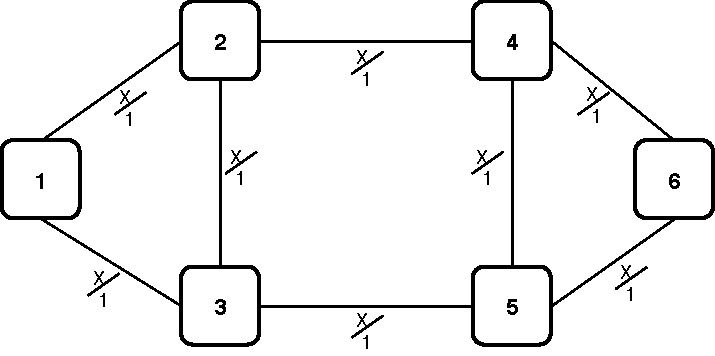
\includegraphics[width=12cm]{sdf/ilp/opaque_survivability/figures/allowed_physical_topology}
\caption{Allowed physical topology. The allowed physical topology is defined by the duct and sites in the field. It is assumed that each duct supports up to 1 bidirectional transmission system and each site supports up to 1 node.}
\label{allowed_physical_medium}
\end{figure}

\begin{figure}[h!]
\centering
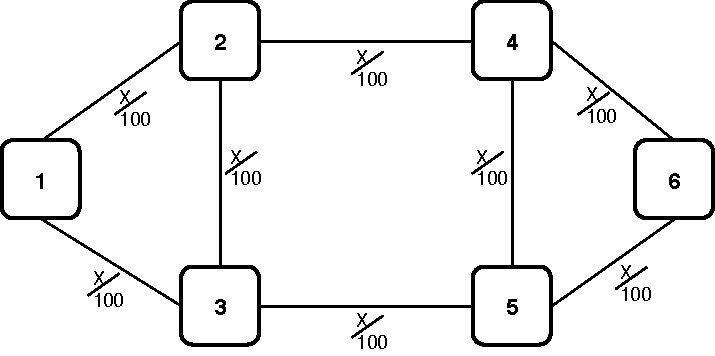
\includegraphics[width=12cm]{sdf/ilp/opaque_survivability/figures/allowed_optical_topology}
\caption{Allowed optical topology. The allowed optical topology is defined by the transport mode (opaque transport mode in this case). It is assumed that each transmission system supports up to 100 optical channels.}
\label{allowed_optical_medium}
\end{figure}
\newpage
\begin{figure}[h!]
\centering
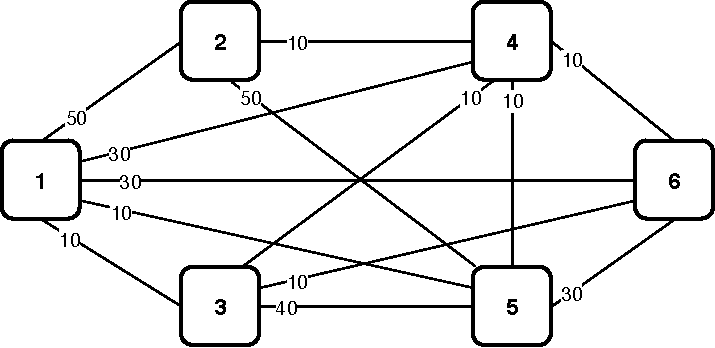
\includegraphics[width=12cm]{sdf/ilp/opaque_survivability/figures/logical_topology_ODU0_medium}
\caption{ODU0 logical topology defined by the ODU0 traffic matrix.}
\label{logical_ODU0_medium}
\end{figure}

\begin{figure}[h!]
\centering
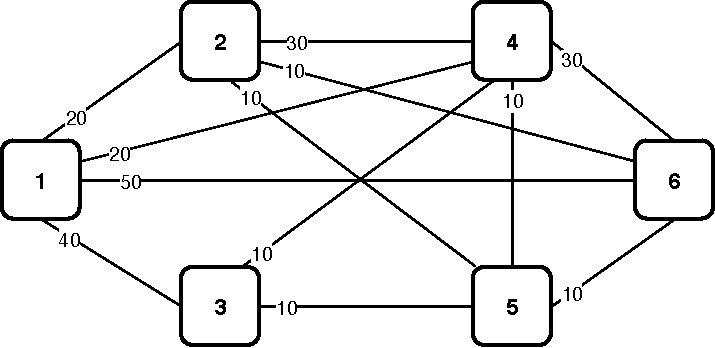
\includegraphics[width=12cm]{sdf/ilp/opaque_survivability/figures/logical_topology_ODU1_medium}
\caption{ODU1 logical topology defined by the ODU1 traffic matrix.}
\label{logical_ODU1_medium}
\end{figure}

\begin{figure}[h!]
\centering
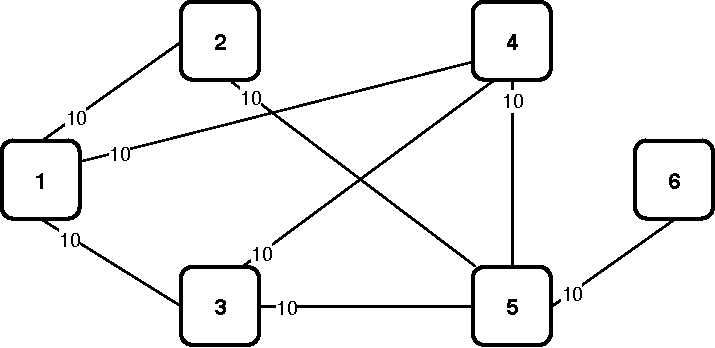
\includegraphics[width=12cm]{sdf/ilp/opaque_survivability/figures/logical_topology_ODU2_medium}
\caption{ODU2 logical topology defined by the ODU2 traffic matrix.}
\label{logical_ODU2_medium}
\end{figure}

\begin{figure}[h!]
\centering
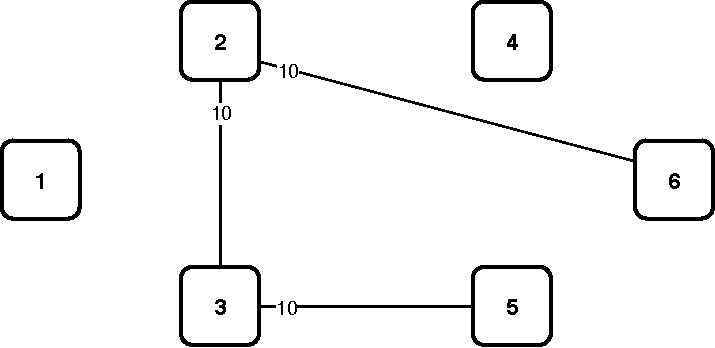
\includegraphics[width=12cm]{sdf/ilp/opaque_survivability/figures/logical_topology_ODU3_medium}
\caption{ODU3 logical topology defined by the ODU3 traffic matrix.}
\label{logical_ODU3_medium}
\end{figure}

\begin{figure}[h!]
\centering
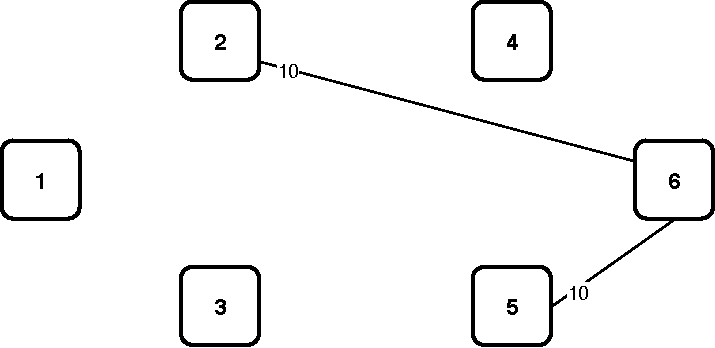
\includegraphics[width=12cm]{sdf/ilp/opaque_survivability/figures/logical_topology_ODU4_medium}
\caption{ODU4 logical topology defined by the ODU4 traffic matrix.}
\label{logical_ODU4_medium}
\end{figure}

\begin{figure}[h!]
\centering
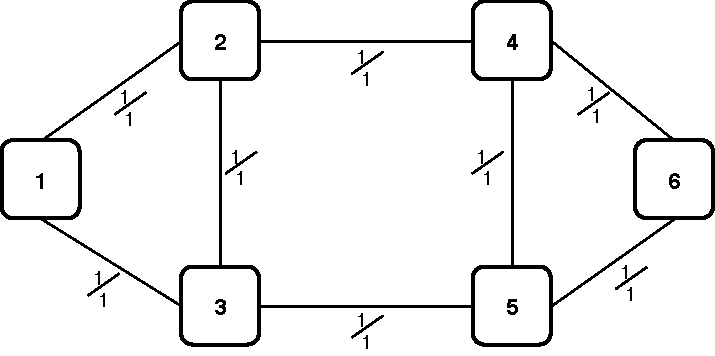
\includegraphics[width=12cm]{sdf/ilp/opaque_survivability/figures/physical_topology}
\caption{Physical topology after dimensioning.}
\label{physical_medium}
\end{figure}
\newpage
\begin{figure}[h!]
\centering
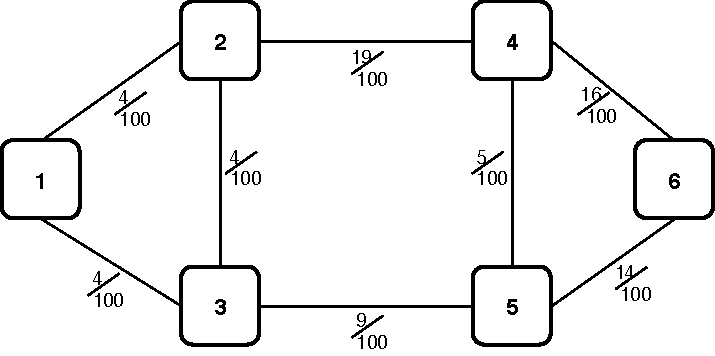
\includegraphics[width=11cm]{sdf/ilp/opaque_survivability/figures/optical_topology_medium}
\caption{Optical topology after dimensioning.}
\label{optical_medium}
\end{figure}

In table \ref{link_opaque_surv_ref_medium} we can see the number of optical channels calculated using \ref{Capex_Link} and \ref{Capex} and the number of amplifiers for each link calculated using \ref{Capex_amplifiers}.

\begin{table}[h!]
\centering
\begin{tabular}{|| c | c | c ||}
 \hline
 \multicolumn{3}{|| c ||}{Information regarding links} \\
 \hline
 \hline
 Bidirectional Link & Optical Channels & Amplifiers\\
 \hline
 Node 1 <-> Node 2 & 4 & 4 \\
 Node 1 <-> Node 3 & 4 & 6 \\
 Node 2 <-> Node 3 & 4 & 0 \\
 Node 2 <-> Node 4 & 19 & 6 \\
 Node 3 <-> Node 5 & 9 & 8 \\
 Node 4 <-> Node 5 & 5 & 1 \\
 Node 4 <-> Node 6 & 16 & 7 \\
 Node 5 <-> Node 6 & 14 & 3 \\
 \hline
\end{tabular}
\caption{Table with information regarding links for opaque mode without survivability.}
\label{link_opaque_surv_ref_medium}
\end{table}

In table \ref{node_opaque_surv_ref_medium} we can see the resulting nodal degree at the physical layer, the number of line ports using \ref{EXC_pexc1_opaque} and the number of tributary ports using \ref{EXC_pexc2_opaque} for each node.

\begin{table}[h!]
\centering
\begin{tabular}{|| c | c | c | c ||}
 \hline
 \multicolumn{4}{|| c ||}{Information regarding nodes} \\
 \hline
 \hline
 Node & Resulting Nodal Degree & Line Ports & Tributary Ports\\
 \hline
 1 & 2 & 8 & 290 \\
 2 & 3 & 27 & 230 \\
 3 & 3 & 17 & 180 \\
 4 & 3 & 40 & 200 \\
 5 & 3 & 28 & 240 \\
 6 & 2 & 30 & 220 \\
\hline
\end{tabular}
\caption{Table with information regarding nodes for opaque mode without survivability.}
\label{node_opaque_surv_ref_medium}
\end{table}

\newpage
Through the information obtained previously on the nodes we can now create tables with detailed information about each node.
In each table with detailed information we can see how many ports are connected to a given node and its bit rate (in relation to the line ports) and how many ports are assigned to each different bit rate (in relation to the tributary ports).\\

\begin{table}[h!]
\centering
\begin{tabular}{|| c | c | c ||}
 \hline
 \multicolumn{3}{|| c ||}{Detailed description of Node 1} \\
 \hline
 \hline
  & Number of total demands & bit rate \\ \hline
\multirow{3}{*}{290 tributary ports} & 130 & ODU0 \\
 & 130 & ODU1 \\
 & 30 & ODU2 \\
 \hline
 \hline
  & Node <-- Optical Channels --> Node & bit rate \\ \hline
\multirow{2}{*}{8 line ports} & 1  <---- 4 ---->  2 & \multirow{2}{*}{100 Gbtis/s} \\
 & 1  <---- 4 ----> 3 & \\
\hline
\end{tabular}
\caption{Table with detailed description of node 1. The number of demands is distributed to the various destination nodes, this distribution can be observed in section \ref{medium_traffic_scenario} .}
\end{table}

\vspace{17pt}
\begin{table}[h!]
\centering
\begin{tabular}{|| c | c | c ||}
 \hline
 \multicolumn{3}{|| c ||}{Detailed description of Node 2} \\
 \hline
 \hline
  & Number of total demands & bit rate \\ \hline
\multirow{5}{*}{230 tributary ports} & 110 & ODU0 \\
 & 70 & ODU1 \\
 & 20 & ODU2 \\
 & 20 & ODU3 \\
 & 10 & ODU4 \\
 \hline
 \hline
  & Node <-- Optical Channels --> Node & bit rate \\ \hline
 \multirow{3}{*}{27 line ports} & 2  <---- 4 ---->  1 & \multirow{3}{*}{100 Gbtis/s}\\
 & 2  <---- 4 ---->  3 & \\
 & 2  <---- 19 ---->  4 & \\
\hline
\end{tabular}
\caption{Table with detailed description of node 2. The number of demands is distributed to the various destination nodes, this distribution can be observed in section \ref{medium_traffic_scenario}.}
\end{table}

\newpage
\begin{table}[h!]
\centering
\begin{tabular}{|| c | c | c ||}
 \hline
 \multicolumn{3}{|| c ||}{Detailed description of Node 3} \\
 \hline
 \hline
  & Number of total demands & bit rate \\ \hline
\multirow{4}{*}{180 tributary ports} & 70 & ODU0 \\
 & 60 & ODU1\\
 & 30 & ODU2\\
 & 20 & ODU3\\
 \hline
 \hline
  & Node <-- Optical Channels --> Node & bit rate \\ \hline
 \multirow{3}{*}{17 line ports} & 3  <---- 4 ---->  1 & \multirow{3}{*}{100 Gbtis/s}\\
 & 3  <---- 4 ---->  2 & \\
 & 3  <---- 9 ---->  5 & \\
\hline
\end{tabular}
\caption{Table with detailed description of node 3. The number of demands is distributed to the various destination nodes, this distribution can be observed in section \ref{medium_traffic_scenario}.}
\end{table}

\begin{table}[h!]
\centering
\begin{tabular}{|| c | c | c ||}
 \hline
 \multicolumn{3}{|| c ||}{Detailed description of Node 4} \\
 \hline
 \hline
  & Number of total demands & bit rate \\ \hline
\multirow{3}{*}{200 tributary ports} & 70 & ODU0 \\
 & 100 & ODU1 \\
 & 30 & ODU2 \\
 \hline
 \hline
  & Node <-- Optical Channels --> Node & bit rate \\ \hline
\multirow{3}{*}{40 line ports} & 4  <---- 19 ---->  2 & \multirow{3}{*}{100 Gbtis/s}\\
 & 4  <---- 5 ---->  5 & \\
 & 4  <---- 16 ---->  6 & \\
\hline
\end{tabular}
\caption{Table with detailed description of node 4. The number of demands is distributed to the various destination nodes, this distribution can be observed in section \ref{medium_traffic_scenario}.}
\end{table}

\begin{table}[h!]
\centering
\begin{tabular}{|| c | c | c ||}
 \hline
 \multicolumn{3}{|| c ||}{Detailed description of Node 5} \\
 \hline
 \hline
  & Number of total demands & bit rate \\ \hline
\multirow{5}{*}{240 tributary ports} & 140 & ODU0 \\
 & 40 & ODU1 \\
 & 40 & ODU2 \\
 & 10 & ODU3 \\
 & 10 & ODU4 \\
 \hline
 \hline
  & Node <-- Optical Channels --> Node & bit rate \\ \hline
 \multirow{3}{*}{28 line ports} & 5  <---- 9 ---->  3 & \multirow{3}{*}{100 Gbtis/s} \\
 & 5  <---- 5 ---->  4 & \\
 & 5  <---- 14 ---->  6 & \\
\hline
\end{tabular}
\caption{Table with detailed description of node 5.}
\end{table}

\newpage
\begin{table}[h!]
\centering
\begin{tabular}{|| c | c | c ||}
 \hline
 \multicolumn{3}{|| c ||}{Detailed description of Node 6} \\
 \hline
 \hline
  & Number of total demands & bit rate \\ \hline
\multirow{5}{*}{220 tributary ports} & 80 & ODU0 \\
 & 100 & ODU1 \\
 & 10 & ODU2 \\
 & 10 & ODU3 \\
 & 20 & ODU4 \\
 \hline
 \hline
  & Node <-- Optical Channels --> Node & bit rate \\ \hline
 \multirow{2}{*}{30 line ports} & 6  <---- 16 ---->  4 & \multirow{2}{*}{100 Gbtis/s} \\
 & 6  <---- 14 ---->  5 & \\
\hline
\end{tabular}
\caption{Table with detailed description of node 6. The number of demands is distributed to the various destination nodes, this distribution can be observed in section \ref{medium_traffic_scenario}.}
\end{table}

\vspace{17pt}
In next step let's focus on the routing information. These paths are bidirectional so the path from one node to another is the same path in the opposite direction. In table \ref{path_opaque_surv_ref_medium} we can see all the routing obtained for all nodes.\\

\begin{table}[h!]
\centering
\begin{tabular}{|| c | c | c | c | c | c | c | c ||}
 \hline
 \multicolumn{8}{|| c ||}{Routing} \\
 \hline
 \hline
 o & d & Links & ODU0 & ODU1 & ODU2 & ODU3 & ODU4 \\
 \hline
 1 & 2 & \{(1,2)\} & 50 & 20 & 10 & 0 & 0 \\ \hline
 1 & 3 & \{(1,3)\} & 10 & 40 & 10 & 0 & 0\\ \hline
 1 & 4 & \{(1,2),(2,4)\} & 30 & 20 & 10 & 0 & 0\\ \hline
 1 & 5 & \{(1,3),(3,5)\} & 10 & 0 & 0 & 0 & 0\\ \hline
 1 & 6 & \{(1,3),(3,5),(5,6)\} & 30 & 50 & 0 & 0 & 0\\ \hline
 2 & 3 & \{(2,3)\} & 0 & 0 & 0 & 10 & 0 \\ \hline
 2 & 4 & \{(2,4)\} & 10 & 30 & 0 & 0 & 0\\ \hline
 2 & 5 & \{(2,4),(4,5)\} & 50 & 10 & 10 & 0 & 0 \\ \hline
 2 & 6 & \{(2,4),(4,6)\} & 0 & 10 & 0 & 10 & 10 \\ \hline
 3 & 4 & \{(3,5),(5,4)\} & 10 & 10 & 10 & 0 & 0 \\ \hline
 3 & 5 & \{(3,5)\} & 40 & 10 & 10 & 10 & 0 \\ \hline
 3 & 6 & \{(3,5),(5,6)\} & 10 & 0 & 0 & 0 & 0\\ \hline
 4 & 5 & \{(4,5)\} & 10 & 10 & 10 & 0 & 0\\ \hline
 4 & 6 & \{(4,6)\} & 10 & 30 & 0 & 0 & 0\\ \hline
 5 & 6 & \{(5,6)\} & 30 & 10 & 10 & 0 & 10\\
 \hline
\end{tabular}
\caption{Table with description of demands routing. We are assuming that between a pair of nodes all demands follow the same route.}
\label{path_opaque_surv_ref_medium}
\end{table}

\newpage
Finally and most importantly through table \ref{scriptopaque_surv_ref_medium} we can see the CAPEX result for this model. This value is obtained using equation \ref{ILPOpaque_CAPEX} and all of the constraints mentioned above.
In table \ref{formulas_opaque} mentioned in previous scenario we can see how all the values were calculated.

\begin{table}[h!]
\centering
\begin{tabular}{|| c | c | c | c | c | c | c ||}
 \hline
 \multicolumn{7}{|| c ||}{CAPEX of the Network} \\
 \hline
 \hline
 \multicolumn{3}{|| c |}{ } & Quantity & Unit Price & Cost & Total \\
 \hline
 \multirow{3}{*}{Link Cost} & \multicolumn{2}{ c |}{OLTs} & 16 & 15 000 \euro & 240 000 \euro & \multirow{3}{*}{75 520 000 \euro} \\ \cline{2-6}
 & \multicolumn{2}{ c |}{100 Gbits/s Transceivers} & 150 & 5 000 \euro/Gbit/s & 75 000 000 \euro & \\ \cline{2-6}
 & \multicolumn{2}{ c |}{Amplifiers} & 70 & 4 000 \euro & 280 000 \euro & \\
 \hline
 \multirow{9}{*}{Node Cost} & \multirow{7}{*}{Electrical} & EXCs & 6 & 10 000 \euro & 60 000 \euro & \multirow{9}{*}{15 085 900 \euro} \\ \cline{3-6}
 & & ODU0 Ports & 600 & 10 \euro/port & 6 000 \euro & \\ \cline{3-6}
 & & ODU1 Ports & 500 & 15 \euro/port & 7 500 \euro & \\ \cline{3-6}
 & & ODU2 Ports & 160 & 30 \euro/port & 4 800 \euro & \\ \cline{3-6}
 & & ODU3 Ports & 60 & 60 \euro/port & 3 600 \euro & \\ \cline{3-6}
 & & ODU4 Ports & 40 & 100 \euro/port & 4 000 \euro & \\ \cline{3-6}
 & & Line Ports & 150 & 100 000 \euro/port & 15 000 000 \euro & \\ \cline{2-6}
 & \multirow{2}{*}{Optical} & OXCs & 0 & 20 000 \euro & 0 \euro & \\ \cline{3-6}
 & & Ports & 0 & 2 500 \euro/port & 0 \euro & \\
 \hline
 \multicolumn{6}{|| c |}{Total Network Cost} & 90 605 900 \euro \\
\hline
\end{tabular}
\caption{Table with detailed description of CAPEX for this scenario.}
\label{scriptopaque_surv_ref_medium}
\end{table}


\textbf{High Traffic Scenario:}\\

In this scenario we have to take into account the traffic calculated in \ref{high_traffic_scenario}. In a first phase we will show the various existing topologies of the network.

\begin{figure}[h!]
\centering
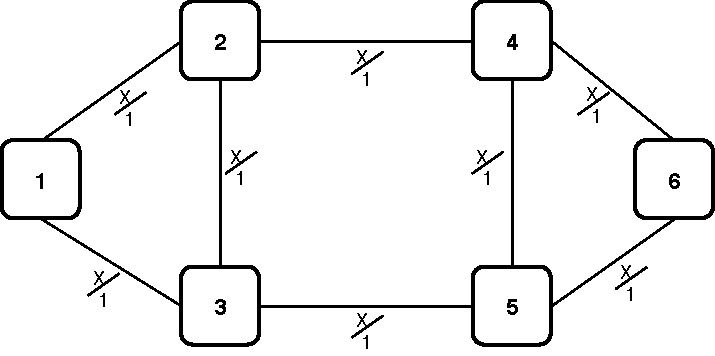
\includegraphics[width=11cm]{sdf/ilp/opaque_survivability/figures/allowed_physical_topology}
\caption{Allowed physical topology. The allowed physical topology is defined by the duct and sites in the field. It is assumed that each duct supports up to 1 bidirectional transmission system and each site supports up to 1 node.}
\label{allowed_physical_high}
\end{figure}
\newpage
\begin{figure}[h!]
\centering
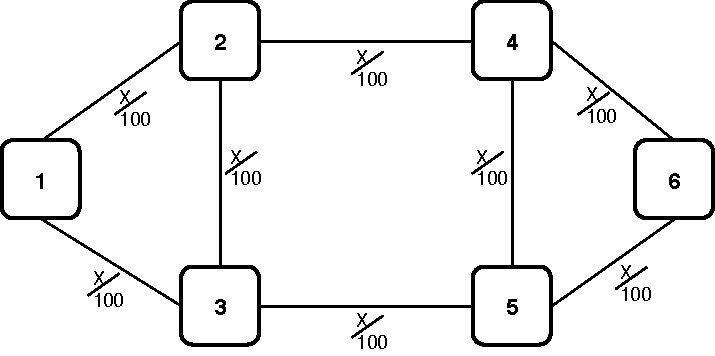
\includegraphics[width=11cm]{sdf/ilp/opaque_survivability/figures/allowed_optical_topology}
\caption{Allowed optical topology. The allowed optical topology is defined by the transport mode (opaque transport mode in this case). It is assumed that each transmission system supports up to 100 optical channels.}
\label{allowed_optical_high}
\end{figure}

\begin{figure}[h!]
\centering
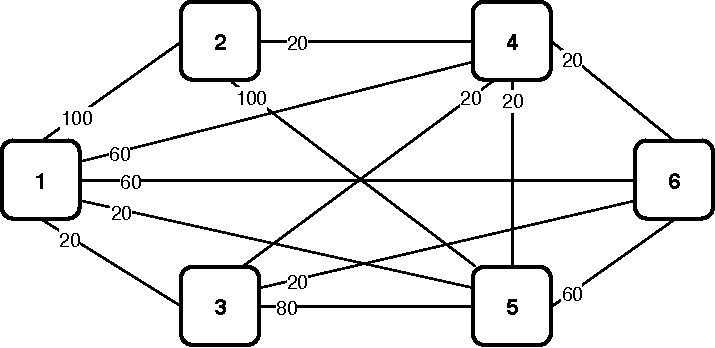
\includegraphics[width=11cm]{sdf/ilp/opaque_survivability/figures/logical_topology_ODU0_high}
\caption{ODU0 logical topology defined by the ODU0 traffic matrix.}
\label{logical_ODU0_high}
\end{figure}

\begin{figure}[h!]
\centering
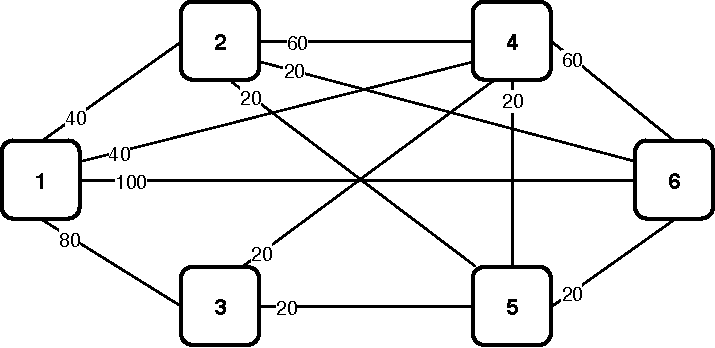
\includegraphics[width=11cm]{sdf/ilp/opaque_survivability/figures/logical_topology_ODU1_high}
\caption{ODU1 logical topology defined by the ODU1 traffic matrix.}
\label{logical_ODU1_high}
\end{figure}
\newpage
\begin{figure}[h!]
\centering
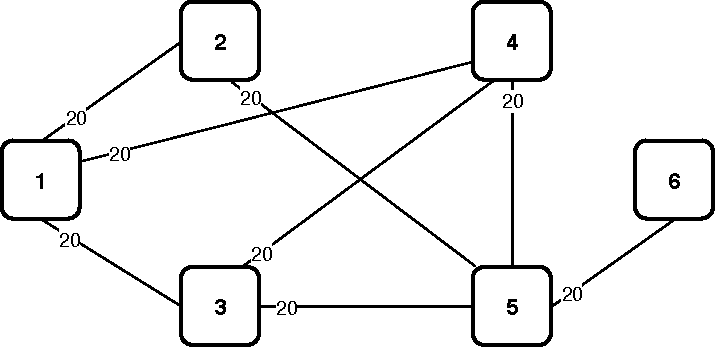
\includegraphics[width=12cm]{sdf/ilp/opaque_survivability/figures/logical_topology_ODU2_high}
\caption{ODU2 logical topology defined by the ODU2 traffic matrix.}
\label{logical_ODU2_high}
\end{figure}

\begin{figure}[h!]
\centering
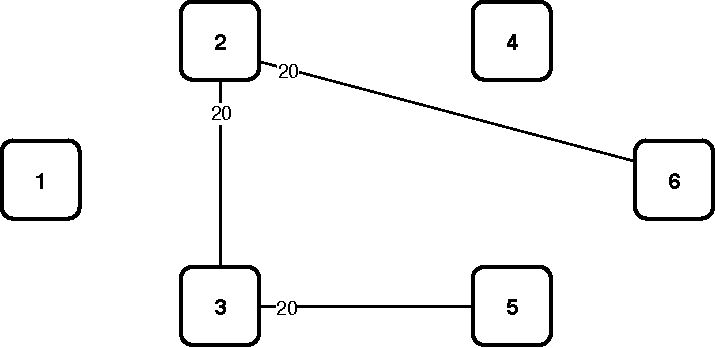
\includegraphics[width=12cm]{sdf/ilp/opaque_survivability/figures/logical_topology_ODU3_high}
\caption{ODU3 logical topology defined by the ODU3 traffic matrix.}
\label{logical_ODU3_high}
\end{figure}

\begin{figure}[h!]
\centering
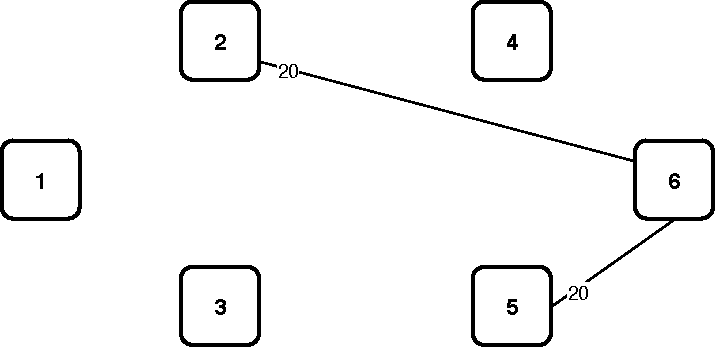
\includegraphics[width=12cm]{sdf/ilp/opaque_survivability/figures/logical_topology_ODU4_high}
\caption{ODU4 logical topology defined by the ODU4 traffic matrix.}
\label{logical_ODU4_high}
\end{figure}
\newpage
\begin{figure}[h!]
\centering
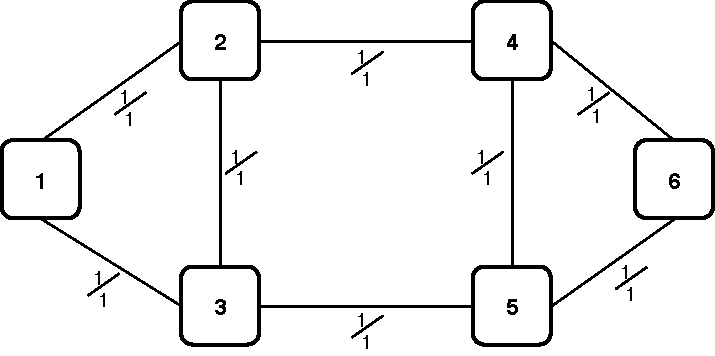
\includegraphics[width=13cm]{sdf/ilp/opaque_survivability/figures/physical_topology}
\caption{Physical topology after dimensioning.}
\label{physical_high}
\end{figure}

\vspace{25pt}

\begin{figure}[h!]
\centering
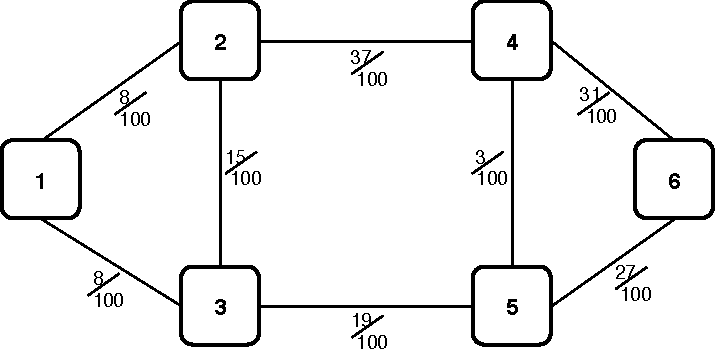
\includegraphics[width=13cm]{sdf/ilp/opaque_survivability/figures/optical_topology_high}
\caption{Optical topology after dimensioning.}
\label{optical_high}
\end{figure}

\newpage
In table \ref{link_opaque_surv_ref_high} we can see the number of optical channels calculated using \ref{Capex_Link} and \ref{Capex} and the number of amplifiers for each link calculated using \ref{amplifiers}.\\

\begin{table}[h!]
\centering
\begin{tabular}{|| c | c | c ||}
 \hline
 \multicolumn{3}{|| c ||}{Information regarding links} \\
 \hline
 \hline
 Bidirectional Link & Optical Channels & Amplifiers\\
 \hline
 Node 1 <-> Node 2 & 8 & 4 \\
 Node 1 <-> Node 3 & 8 & 6 \\
 Node 2 <-> Node 3 & 15 & 0 \\
 Node 2 <-> Node 4 & 37 & 6 \\
 Node 3 <-> Node 5 & 19 & 8 \\
 Node 4 <-> Node 5 & 3 & 1 \\
 Node 4 <-> Node 6 & 31 & 7 \\
 Node 5 <-> Node 6 & 27 & 3 \\
 \hline
\end{tabular}
\caption{Table with information regarding links for opaque mode without survivability.}
\label{link_opaque_surv_ref_high}
\end{table}

\vspace{13pt}
In table \ref{node_opaque_surv_ref_high} we can see the resulting nodal degree at the physical layer, calculated based on the number of connections that the node in question performs, the number of line ports calculated using \ref{EXC_pexc1_opaque} and the number of tributary ports calculated using \ref{EXC_pexc2_opaque} for each node.\\

\begin{table}[h!]
\centering
\begin{tabular}{|| c | c | c | c ||}
 \hline
 \multicolumn{4}{|| c ||}{Information regarding nodes} \\
 \hline
 \hline
 Node & Resulting Nodal Degree & Line Ports & Tributary Ports\\
 \hline
 1 & 2 & 16 & 580 \\
 2 & 3 & 60 & 460 \\
 3 & 3 & 42 & 360 \\
 4 & 3 & 71 & 400 \\
 5 & 3 & 49 & 480 \\
 6 & 2 & 58 & 440 \\
\hline
\end{tabular}
\caption{Table with information regarding nodes for opaque mode without survivability.}
\label{node_opaque_surv_ref_high}
\end{table}

\vspace{13pt}
In each table mentioned next with detailed information we can see how many ports are connected to a given node and its bit rate (in relation to the line ports) and how many ports are assigned to each different bit rate (in relation to the tributary ports).\\
\newpage
\begin{table}[h!]
\centering
\begin{tabular}{|| c | c | c ||}
 \hline
 \multicolumn{3}{|| c ||}{Detailed description of Node 1} \\
 \hline
 \hline
  & Number of total demands & bit rate \\ \hline
\multirow{3}{*}{580 tributary ports} & 260 & ODU0 \\
 & 260 & ODU1 \\
 & 60 & ODU2 \\
 \hline
 \hline
  & Node <-- Optical Channels --> Node & bit rate \\ \hline
\multirow{2}{*}{16 line ports} & 1  <---- 8 ---->  2 & \multirow{2}{*}{100 Gbtis/s} \\
 & 1  <---- 8 ---->  3 & \\
\hline
\end{tabular}
\caption{Table with detailed description of node 1. The number of demands is distributed to the various destination nodes, this distribution can be observed in section \ref{high_traffic_scenario} .}
\end{table}

\begin{table}[h!]
\centering
\begin{tabular}{|| c | c | c ||}
 \hline
 \multicolumn{3}{|| c ||}{Detailed description of Node 2} \\
 \hline
 \hline
  & Number of total demands & bit rate \\ \hline
\multirow{5}{*}{460 tributary ports} & 220 & ODU0 \\
 & 140 & ODU1 \\
 & 40 & ODU2 \\
 & 40 & ODU3 \\
 & 20 & ODU4 \\
\hline
\hline
 & Node <-- Optical Channels --> Node & bit rate \\ \hline
 \multirow{3}{*}{60 line ports} & 2  <---- 8 ---->  1 & \multirow{3}{*}{100 Gbtis/s}\\
 & 2  <---- 15 ---->  3 & \\
 & 2  <---- 37 ---->  4 & \\
 \hline
\end{tabular}
\caption{Table with detailed description of node 2. The number of demands is distributed to the various destination nodes, this distribution can be observed in section \ref{high_traffic_scenario}.}
\end{table}

\begin{table}[h!]
\centering
\begin{tabular}{|| c | c | c ||}
 \hline
 \multicolumn{3}{|| c ||}{Detailed description of Node 3} \\
 \hline
 \hline
  & Number of total demands & bit rate \\ \hline
\multirow{4}{*}{360 tributary ports} & 140 & ODU0 \\
 & 120 & ODU1\\
 & 60 & ODU2\\
 & 40 & ODU3\\
 \hline
 \hline
  & Node <-- Optical Channels --> Node & bit rate \\ \hline
 \multirow{3}{*}{42 line ports} & 3  <---- 8 ---->  1 & \multirow{3}{*}{100 Gbtis/s}\\
 & 3  <---- 15 ---->  2 & \\
 & 3  <---- 19 ---->  5 & \\
\hline
\end{tabular}
\caption{Table with detailed description of node 3. The number of demands is distributed to the various destination nodes, this distribution can be observed in section \ref{high_traffic_scenario}.}
\end{table}

\newpage
\begin{table}[h!]
\centering
\begin{tabular}{|| c | c | c ||}
 \hline
 \multicolumn{3}{|| c ||}{Detailed description of Node 4} \\
 \hline
 \hline
  & Number of total demands & bit rate \\ \hline
\multirow{3}{*}{400 tributary ports} & 140 & ODU0 \\
 & 200 & ODU1 \\
 & 60 & ODU2 \\
 \hline
 \hline
  & Node <-- Optical Channels --> Node & bit rate \\ \hline
\multirow{3}{*}{71 line ports} & 4  <---- 37 ---->  2 & \multirow{3}{*}{100 Gbtis/s}\\
 & 4  <---- 3 ---->  5 & \\
 & 4  <---- 31 ---->  6 & \\
\hline
\end{tabular}
\caption{Table with detailed description of node 4. The number of demands is distributed to the various destination nodes, this distribution can be observed in section \ref{high_traffic_scenario}.}
\end{table}

\begin{table}[h!]
\centering
\begin{tabular}{|| c | c | c ||}
 \hline
 \multicolumn{3}{|| c ||}{Detailed description of Node 5} \\
 \hline
 \hline
  & Number of total demands & bit rate \\ \hline
\multirow{5}{*}{480 tributary ports} & 280 & ODU0 \\
 & 80 & ODU1 \\
 & 80 & ODU2 \\
 & 20 & ODU3 \\
 & 20 & ODU4 \\
 \hline
 \hline
  & Node <-- Optical Channels --> Node & bit rate \\ \hline
 \multirow{3}{*}{49 line ports} & 5  <---- 19 ---->  3 & \multirow{3}{*}{100 Gbtis/s} \\
 & 5  <---- 3 ---->  4 & \\
 & 5  <---- 27 ---->  6 & \\
\hline
\end{tabular}
\caption{Table with detailed description of node 5. The number of demands is distributed to the various destination nodes, this distribution can be observed in section \ref{high_traffic_scenario}.}
\end{table}

\begin{table}[h!]
\centering
\begin{tabular}{|| c | c | c ||}
 \hline
 \multicolumn{3}{|| c ||}{Detailed description of Node 6} \\
 \hline
 \hline
  & Number of total demands & bit rate \\ \hline
\multirow{5}{*}{440 tributary ports} & 160 & ODU0 \\
 & 200 & ODU1 \\
 & 20 & ODU2 \\
 & 20 & ODU3 \\
 & 40 & ODU4 \\
 \hline
 \hline
  & Node <-- Optical Channels --> Node & bit rate \\ \hline
 \multirow{2}{*}{58 line ports} & 6  <---- 31 ---->  4 & \multirow{2}{*}{100 Gbtis/s} \\
 & 6  <---- 27 ---->  5 & \\
\hline
\end{tabular}
\caption{Table with detailed description of node 6.}
\end{table}

\newpage
In next step let's focus on the routing information. These paths are bidirectional so the path from one node to another is the same path in the opposite direction. In table \ref{path_opaque_surv_ref_high} we can see all the routing obtained for all nodes.\\

\begin{table}[h!]
\centering
\begin{tabular}{|| c | c | c | c | c | c | c | c ||}
 \hline
 \multicolumn{8}{|| c ||}{Routing} \\
 \hline
 \hline
 o & d & Links & ODU0 & ODU1 & ODU2 & ODU3 & ODU4 \\
 \hline
 1 & 2 & \{(1,2)\} & 100 & 40 & 20 & 0 & 0 \\ \hline
 1 & 3 & \{(1,3)\} & 20 & 80 & 20 & 0 & 0\\ \hline
 1 & 4 & \{(1,2),(2,4)\} & 60 & 40 & 20 & 0 & 0\\ \hline
 1 & 5 & \{(1,3),(3,5)\} & 20 & 0 & 0 & 0 & 0\\ \hline
 1 & 6 & \{(1,3),(3,5),(5,6)\} & 60 & 100 & 0 & 0 & 0\\ \hline
 2 & 3 & \{(2,3)\} & 0 & 0 & 0 & 20 & 0 \\ \hline
 2 & 4 & \{(2,4)\} & 20 & 60 & 0 & 0 & 0\\ \hline
 2 & 5 & \{(2,3),(3,5)\} & 100 & 20 & 20 & 0 & 0 \\ \hline
 2 & 6 & \{(2,4),(4,6)\} & 0 & 20 & 0 & 20 & 20 \\ \hline
 3 & 4 & \{(3,2),(2,4)\} & 20 & 20 & 20 & 0 & 0 \\ \hline
 3 & 5 & \{(3,5)\} & 80 & 20 & 20 & 20 & 0 \\ \hline
 3 & 6 & \{(3,5),(5,6)\} & 20 & 0 & 0 & 0 & 0\\ \hline
 4 & 5 & \{(4,5)\} & 20 & 20 & 20 & 0 & 0\\ \hline
 4 & 6 & \{(4,6)\} & 20 & 60 & 0 & 0 & 0\\ \hline
 5 & 6 & \{(5,6)\} & 60 & 20 & 20 & 0 & 20\\
 \hline
\end{tabular}
\caption{Table with description of demands routing. We are assuming that between a pair of nodes all demands follow the same route.}
\label{path_opaque_surv_ref_high}
\end{table}

\vspace{13pt}
Finally and most importantly through table \ref{scriptopaque_surv_ref_high} we can see the CAPEX result for this model. This value is obtained using equation \ref{ILPOpaque_CAPEX} and all of the constraints mentioned above.
In table \ref{formulas_opaque} mentioned in previous scenario we can see how all the values were calculated.\\
\newpage
\begin{table}[h!]
\centering
\begin{tabular}{|| c | c | c | c | c | c | c ||}
 \hline
 \multicolumn{7}{|| c ||}{CAPEX of the Network} \\
 \hline
 \hline
 \multicolumn{3}{|| c |}{ } & Quantity & Unit Price & Cost & Total \\
 \hline
 \multirow{3}{*}{Link Cost} & \multicolumn{2}{ c |}{OLTs} & 16 & 15 000 \euro & 240 000 \euro & \multirow{3}{*}{148 520 000 \euro} \\ \cline{2-6}
 & \multicolumn{2}{ c |}{100 Gbits/s Transceivers} & 296 & 5 000 \euro/Gbit/s & 148 000 000 \euro & \\ \cline{2-6}
 & \multicolumn{2}{ c |}{Amplifiers} & 70 & 4 000 \euro & 280 000 \euro & \\
 \hline
 \multirow{9}{*}{Node Cost} & \multirow{7}{*}{Electrical} & EXCs & 6 & 10 000 \euro & 60 000 \euro & \multirow{9}{*}{29 711 800 \euro} \\ \cline{3-6}
 & & ODU0 Ports & 1 200 & 10 \euro/port & 12 000 \euro & \\ \cline{3-6}
 & & ODU1 Ports & 1 000 & 15 \euro/port & 15 000 \euro & \\ \cline{3-6}
 & & ODU2 Ports & 320 & 30 \euro/port & 9 600 \euro & \\ \cline{3-6}
 & & ODU3 Ports & 120 & 60 \euro/port & 7 200 \euro & \\ \cline{3-6}
 & & ODU4 Ports & 80 & 100 \euro/port & 8 000 \euro & \\ \cline{3-6}
 & & Line Ports & 296 & 100 000 \euro/port & 29 600 000 \euro & \\ \cline{2-6}
 & \multirow{2}{*}{Optical} & OXCs & 0 & 20 000 \euro & 0 \euro & \\ \cline{3-6}
 & & Ports & 0 & 2 500 \euro/port & 0 \euro & \\
 \hline
 \multicolumn{6}{|| c |}{Total Network Cost} & 178 231 800 \euro \\
\hline
\end{tabular}
\caption{Table with detailed description of CAPEX for this scenario.}
\label{scriptopaque_surv_ref_high}
\end{table}

\vspace{13pt}
\subsubsection{Conclusions}

Once we have obtained the results for all the scenarios we will now draw some conclusions about these results. For a better analysis of the results will be created the table \ref{table_comparative_opaque_surv} with the number of line ports, tributary ports and transceivers because they are important values for the cost of CAPEX, the cost of links, the cost of nodes and finally the cost of CAPEX.\\

\begin{table}[h!]
\centering
\begin{tabular}{| c | c | c | c |}
 \hline
  & Low Traffic & Medium Traffic  & High Traffic \\
 \hline\hline
 Traffic (Gbit/s) & 500 & 5 000 & 10 000 \\ \hline
 Bidirectional Links used & 6 & 8 & 8 \\ \hline
 Number of Line ports & 18 & 150 & 296 \\ \hline
 Number of Tributary ports & 136 & 1 360 & 2 720 \\ \hline
 Number of Transceivers & 18 & 150 & 296 \\ \hline
 Link Cost & 9 404 000 \euro & 75 520 000 \euro & 148 520 000 \euro \\ \hline
 Node Cost & 1 862 590 \euro & 15 085 900 \euro & 29 711 800 \euro \\ \hline
 CAPEX & \textbf{11 266 590 \euro} & \textbf{90 605 900 \euro} & \textbf{178 231 800 \euro} \\ \hline
 CAPEX/Gbit/s & \textbf{22 533 \euro/Gbit/s} & \textbf{18 121 \euro/Gbit/s} & \textbf{17 823 \euro/Gbit/s}\\
 \hline
\end{tabular}
\caption{Table with the various CAPEX values obtained in the different traffic scenarios.}
\label{table_comparative_opaque_surv}
\end{table}

\newpage
Looking at the previous table we can make some comparisons between the several scenarios:

\begin{itemize}
  \item Low traffic scenario uses less links than the other two scenarios. This happens because as it has low traffic it is possible to carry this traffic throughout the network without having to use all available links;
  \item Comparing the low traffic scenario with the others we can see that despite having an increase of factor ten (medium scenario) and factor twenty (high scenario) the same increase does not occur in the final cost (it is lower). This happens because the number of transceivers is smaller than expected (medium scenario would be expected 180 and high scenario would be expected 360);
  \item Comparing the medium traffic scenario with the high traffic scenario we can see that the increase of the factor is double and in the final cost this factor is very close but still inferior. Again this happens because the number of transceivers is lower but very close to the expected (high scenario would be expected 300).
  \item Comparing the cost with traffic we see that as traffic increases the cost per traffic decreases. Soon we can conclude that it becomes more expensive a scenario of low traffic than a scenario of high traffic.
\end{itemize}


\vspace{13pt}
\subsubsection{Opens Issues}

The creation of this model for any scenario, started with some considerations and some open issues being:

\begin{itemize}
  \item Allow blocking.
  \subitem The presented model assume that the solution is possible or impossible, does not support a partial solution where some demands are not routed (are blocked).
  \item Allow multiple transmission system.
  \subitem The presented model for each link only supports one transmission system.
  \item Allowing multi-path routing.
  \subitem In the presented model all demands sharing the same end nodes have to follow the same path.
\end{itemize}

